%% bare_conf.tex
%% V1.4b
%% 2015/08/26
%% by Michael Shell
%% See:
%% http://www.michaelshell.org/
%% for current contact information.
%%
%% This is a skeleton file demonstrating the use of IEEEtran.cls
%% (requires IEEEtran.cls version 1.8b or later) with an IEEE
%% conference paper.
%%
%% Support sites:
%% http://www.michaelshell.org/tex/ieeetran/
%% http://www.ctan.org/pkg/ieeetran
%% and
%% http://www.ieee.org/

%%*************************************************************************
%% Legal Notice:
%% This code is offered as-is without any warranty either expressed or
%% implied; without even the implied warranty of MERCHANTABILITY or
%% FITNESS FOR A PARTICULAR PURPOSE! 
%% User assumes all risk.
%% In no event shall the IEEE or any contributor to this code be liable for
%% any damages or losses, including, but not limited to, incidental,
%% consequential, or any other damages, resulting from the use or misuse
%% of any information contained here.
%%
%% All comments are the opinions of their respective authors and are not
%% necessarily endorsed by the IEEE.
%%
%% This work is distributed under the LaTeX Project Public License (LPPL)
%% ( http://www.latex-project.org/ ) version 1.3, and may be freely used,
%% distributed and modified. A copy of the LPPL, version 1.3, is included
%% in the base LaTeX documentation of all distributions of LaTeX released
%% 2003/12/01 or later.
%% Retain all contribution notices and credits.
%% ** Modified files should be clearly indicated as such, including  **
%% ** renaming them and changing author support contact information. **
%%*************************************************************************


% *** Authors should verify (and, if needed, correct) their LaTeX system  ***
% *** with the testflow diagnostic prior to trusting their LaTeX platform ***
% *** with production work. The IEEE's font choices and paper sizes can   ***
% *** trigger bugs that do not appear when using other class files.       ***                          ***
% The testflow support page is at:
% http://www.michaelshell.org/tex/testflow/



\documentclass[conference]{IEEEtran}
% Some Computer Society conferences also require the compsoc mode option,
% but others use the standard conference format.
%
% If IEEEtran.cls has not been installed into the LaTeX system files,
% manually specify the path to it like:
% \documentclass[conference]{../sty/IEEEtran}





% Some very useful LaTeX packages include:
% (uncomment the ones you want to load)


% *** MISC UTILITY PACKAGES ***
%
%\usepackage{ifpdf}
% Heiko Oberdiek's ifpdf.sty is very useful if you need conditional
% compilation based on whether the output is pdf or dvi.
% usage:
% \ifpdf
%   % pdf code
% \else
%   % dvi code
% \fi
% The latest version of ifpdf.sty can be obtained from:
% http://www.ctan.org/pkg/ifpdf
% Also, note that IEEEtran.cls V1.7 and later provides a builtin
% \ifCLASSINFOpdf conditional that works the same way.
% When switching from latex to pdflatex and vice-versa, the compiler may
% have to be run twice to clear warning/error messages.






% *** CITATION PACKAGES ***
%
%\usepackage{cite}
% cite.sty was written by Donald Arseneau
% V1.6 and later of IEEEtran pre-defines the format of the cite.sty package
% \cite{} output to follow that of the IEEE. Loading the cite package will
% result in citation numbers being automatically sorted and properly
% "compressed/ranged". e.g., [1], [9], [2], [7], [5], [6] without using
% cite.sty will become [1], [2], [5]--[7], [9] using cite.sty. cite.sty's
% \cite will automatically add leading space, if needed. Use cite.sty's
% noadjust option (cite.sty V3.8 and later) if you want to turn this off
% such as if a citation ever needs to be enclosed in parenthesis.
% cite.sty is already installed on most LaTeX systems. Be sure and use
% version 5.0 (2009-03-20) and later if using hyperref.sty.
% The latest version can be obtained at:
% http://www.ctan.org/pkg/cite
% The documentation is contained in the cite.sty file itself.






% *** GRAPHICS RELATED PACKAGES ***
%
\ifCLASSINFOpdf
  % \usepackage[pdftex]{graphicx}
  % declare the path(s) where your graphic files are
  % \graphicspath{{../pdf/}{../jpeg/}}
  % and their extensions so you won't have to specify these with
  % every instance of \includegraphics
  % \DeclareGraphicsExtensions{.pdf,.jpeg,.png}
\else
  % or other class option (dvipsone, dvipdf, if not using dvips). graphicx
  % will default to the driver specified in the system graphics.cfg if no
  % driver is specified.
  % \usepackage[dvips]{graphicx}
  % declare the path(s) where your graphic files are
  % \graphicspath{{../eps/}}
  % and their extensions so you won't have to specify these with
  % every instance of \includegraphics
  % \DeclareGraphicsExtensions{.eps}
\fi
% graphicx was written by David Carlisle and Sebastian Rahtz. It is
% required if you want graphics, photos, etc. graphicx.sty is already
% installed on most LaTeX systems. The latest version and documentation
% can be obtained at: 
% http://www.ctan.org/pkg/graphicx
% Another good source of documentation is "Using Imported Graphics in
% LaTeX2e" by Keith Reckdahl which can be found at:
% http://www.ctan.org/pkg/epslatex
%
% latex, and pdflatex in dvi mode, support graphics in encapsulated
% postscript (.eps) format. pdflatex in pdf mode supports graphics
% in .pdf, .jpeg, .png and .mps (metapost) formats. Users should ensure
% that all non-photo figures use a vector format (.eps, .pdf, .mps) and
% not a bitmapped formats (.jpeg, .png). The IEEE frowns on bitmapped formats
% which can result in "jaggedy"/blurry rendering of lines and letters as
% well as large increases in file sizes.
%
% You can find documentation about the pdfTeX application at:
% http://www.tug.org/applications/pdftex





% *** MATH PACKAGES ***
%
%\usepackage{amsmath}
% A popular package from the American Mathematical Society that provides
% many useful and powerful commands for dealing with mathematics.
%
% Note that the amsmath package sets \interdisplaylinepenalty to 10000
% thus preventing page breaks from occurring within multiline equations. Use:
%\interdisplaylinepenalty=2500
% after loading amsmath to restore such page breaks as IEEEtran.cls normally
% does. amsmath.sty is already installed on most LaTeX systems. The latest
% version and documentation can be obtained at:
% http://www.ctan.org/pkg/amsmath





% *** SPECIALIZED LIST PACKAGES ***
%
%\usepackage{algorithmic}
% algorithmic.sty was written by Peter Williams and Rogerio Brito.
% This package provides an algorithmic environment fo describing algorithms.
% You can use the algorithmic environment in-text or within a figure
% environment to provide for a floating algorithm. Do NOT use the algorithm
% floating environment provided by algorithm.sty (by the same authors) or
% algorithm2e.sty (by Christophe Fiorio) as the IEEE does not use dedicated
% algorithm float types and packages that provide these will not provide
% correct IEEE style captions. The latest version and documentation of
% algorithmic.sty can be obtained at:
% http://www.ctan.org/pkg/algorithms
% Also of interest may be the (relatively newer and more customizable)
% algorithmicx.sty package by Szasz Janos:
% http://www.ctan.org/pkg/algorithmicx
\usepackage{graphicx}
\graphicspath{{Resources/Figures/MultiPurpose/}}
\usepackage{algpseudocode}
\usepackage{algorithm}
\usepackage[usenames,dvipsnames]{xcolor}
\usepackage{tabu}
\usepackage{colortbl}
\usepackage{xcolor}
\usepackage[lofdepth=1,lotdepth]{subfig}
\usepackage{grfext}
\PrependGraphicsExtensions*{.pdf,.PDF}
\usepackage{amsmath}

% *** ALIGNMENT PACKAGES ***
%
%\usepackage{array}
% Frank Mittelbach's and David Carlisle's array.sty patches and improves
% the standard LaTeX2e array and tabular environments to provide better
% appearance and additional user controls. As the default LaTeX2e table
% generation code is lacking to the point of almost being broken with
% respect to the quality of the end results, all users are strongly
% advised to use an enhanced (at the very least that provided by array.sty)
% set of table tools. array.sty is already installed on most systems. The
% latest version and documentation can be obtained at:
% http://www.ctan.org/pkg/array


% IEEEtran contains the IEEEeqnarray family of commands that can be used to
% generate multiline equations as well as matrices, tables, etc., of high
% quality.




% *** SUBFIGURE PACKAGES ***
%\ifCLASSOPTIONcompsoc
%  \usepackage[caption=false,font=normalsize,labelfont=sf,textfont=sf]{subfig}
%\else
%  \usepackage[caption=false,font=footnotesize]{subfig}
%\fi
% subfig.sty, written by Steven Douglas Cochran, is the modern replacement
% for subfigure.sty, the latter of which is no longer maintained and is
% incompatible with some LaTeX packages including fixltx2e. However,
% subfig.sty requires and automatically loads Axel Sommerfeldt's caption.sty
% which will override IEEEtran.cls' handling of captions and this will result
% in non-IEEE style figure/table captions. To prevent this problem, be sure
% and invoke subfig.sty's "caption=false" package option (available since
% subfig.sty version 1.3, 2005/06/28) as this is will preserve IEEEtran.cls
% handling of captions.
% Note that the Computer Society format requires a larger sans serif font
% than the serif footnote size font used in traditional IEEE formatting
% and thus the need to invoke different subfig.sty package options depending
% on whether compsoc mode has been enabled.
%
% The latest version and documentation of subfig.sty can be obtained at:
% http://www.ctan.org/pkg/subfig




% *** FLOAT PACKAGES ***
%
%\usepackage{fixltx2e}
% fixltx2e, the successor to the earlier fix2col.sty, was written by
% Frank Mittelbach and David Carlisle. This package corrects a few problems
% in the LaTeX2e kernel, the most notable of which is that in current
% LaTeX2e releases, the ordering of single and double column floats is not
% guaranteed to be preserved. Thus, an unpatched LaTeX2e can allow a
% single column figure to be placed prior to an earlier double column
% figure.
% Be aware that LaTeX2e kernels dated 2015 and later have fixltx2e.sty's
% corrections already built into the system in which case a warning will
% be issued if an attempt is made to load fixltx2e.sty as it is no longer
% needed.
% The latest version and documentation can be found at:
% http://www.ctan.org/pkg/fixltx2e


%\usepackage{stfloats}
% stfloats.sty was written by Sigitas Tolusis. This package gives LaTeX2e
% the ability to do double column floats at the bottom of the page as well
% as the top. (e.g., "\begin{figure*}[!b]" is not normally possible in
% LaTeX2e). It also provides a command:
%\fnbelowfloat
% to enable the placement of footnotes below bottom floats (the standard
% LaTeX2e kernel puts them above bottom floats). This is an invasive package
% which rewrites many portions of the LaTeX2e float routines. It may not work
% with other packages that modify the LaTeX2e float routines. The latest
% version and documentation can be obtained at:
% http://www.ctan.org/pkg/stfloats
% Do not use the stfloats baselinefloat ability as the IEEE does not allow
% \baselineskip to stretch. Authors submitting work to the IEEE should note
% that the IEEE rarely uses double column equations and that authors should try
% to avoid such use. Do not be tempted to use the cuted.sty or midfloat.sty
% packages (also by Sigitas Tolusis) as the IEEE does not format its papers in
% such ways.
% Do not attempt to use stfloats with fixltx2e as they are incompatible.
% Instead, use Morten Hogholm'a dblfloatfix which combines the features
% of both fixltx2e and stfloats:
%
% \usepackage{dblfloatfix}
% The latest version can be found at:
% http://www.ctan.org/pkg/dblfloatfix




% *** PDF, URL AND HYPERLINK PACKAGES ***
%
%\usepackage{url}
% url.sty was written by Donald Arseneau. It provides better support for
% handling and breaking URLs. url.sty is already installed on most LaTeX
% systems. The latest version and documentation can be obtained at:
% http://www.ctan.org/pkg/url
% Basically, \url{my_url_here}.




% *** Do not adjust lengths that control margins, column widths, etc. ***
% *** Do not use packages that alter fonts (such as pslatex).         ***
% There should be no need to do such things with IEEEtran.cls V1.6 and later.
% (Unless specifically asked to do so by the journal or conference you plan
% to submit to, of course. )


% correct bad hyphenation here
\hyphenation{op-tical net-works semi-conduc-tor}


\begin{document}
%
% paper title
% Titles are generally capitalized except for words such as a, an, and, as,
% at, but, by, for, in, nor, of, on, or, the, to and up, which are usually
% not capitalized unless they are the first or last word of the title.
% Linebreaks \\ can be used within to get better formatting as desired.
% Do not put math or special symbols in the title.
\title{Self-Organizing Autonomic Computing Systems for Cloud Resource Management}


% author names and affiliations
% use a multiple column layout for up to three different
% affiliations
\author{\IEEEauthorblockN{Bogdan Solomon\IEEEauthorrefmark{1}, Dan Ionescu\IEEEauthorrefmark{2}, Cristian Gadea\IEEEauthorrefmark{3}}
\IEEEauthorblockA{School of Electrical Engineering and Computer Science\\
University of Ottawa\\
Ottawa, ON, Canada\\
Email: \IEEEauthorrefmark{1}bsolomon@ncct.uottawa.ca, \IEEEauthorrefmark{2}dan@ncct.uottawa.ca, \IEEEauthorrefmark{3}cgadea@ncct.uottawa.ca}
}

% conference papers do not typically use \thanks and this command
% is locked out in conference mode. If really needed, such as for
% the acknowledgment of grants, issue a \IEEEoverridecommandlockouts
% after \documentclass

% for over three affiliations, or if they all won't fit within the width
% of the page, use this alternative format:
% 
%\author{\IEEEauthorblockN{Michael Shell\IEEEauthorrefmark{1},
%Homer Simpson\IEEEauthorrefmark{2},
%James Kirk\IEEEauthorrefmark{3}, 
%Montgomery Scott\IEEEauthorrefmark{3} and
%Eldon Tyrell\IEEEauthorrefmark{4}}
%\IEEEauthorblockA{\IEEEauthorrefmark{1}School of Electrical and Computer Engineering\\
%Georgia Institute of Technology,
%Atlanta, Georgia 30332--0250\\ Email: see http://www.michaelshell.org/contact.html}
%\IEEEauthorblockA{\IEEEauthorrefmark{2}Twentieth Century Fox, Springfield, USA\\
%Email: homer@thesimpsons.com}
%\IEEEauthorblockA{\IEEEauthorrefmark{3}Starfleet Academy, San Francisco, California 96678-2391\\
%Telephone: (800) 555--1212, Fax: (888) 555--1212}
%\IEEEauthorblockA{\IEEEauthorrefmark{4}Tyrell Inc., 123 Replicant Street, Los Angeles, California 90210--4321}}




% use for special paper notices
%\IEEEspecialpapernotice{(Invited Paper)}




% make the title area
\maketitle

% As a general rule, do not put math, special symbols or citations
% in the abstract
\begin{abstract}
In recent years, a great deal of research has been undertaken in the area of automating the enterprise IT Infrastructure. For enterprises with a large number of computers, the IT Infrastructure represents a considerable amount of the enterprise budget assigned to its operation. Autonomic Computing Systems are systems which were created to correct and optimize the IT infrastructure's own self-functioning by executing corrective operations without any need for human intervention. Applications of autonomic systems range from usage optimization for clusters of servers or virtual machines, to error prevention and error recovery for web applications. In most cases where autonomic computing systems have been developed, this was achieved by the addition of external global controllers monitoring the subsystems of the enterprise IT Infrastructure, determining where changes should be made and applying appropriate commands to implement these changes. At the same time, the software industry has seen an explosion in the usage of cloud based services. By moving services in the cloud, companies can decrease the IT budget such that they only use the resources which are needed, when they are needed. Furthermore, services deployed in the cloud can be distributed geographically across multiple datacenters such that users obtain a higher quality of service by connecting to a closer datacenter. Self-Organizing systems are systems which reach a global desired state without the use of any central authority. Such systems are better suited to manage a cloud of servers than a centralized controller as they scale better when the controlled system is scaled also. In this paper, an autonomic system based on a self-organizing architecture is introduced. The system is applied to the self-optimization of a web-based real-time collaborative application running on a geographically distributed cloud. Experiments and simulations with the self-organizing, self-optimizing autonomic computing methodology are given to support the design and the implementation described.
\end{abstract}

% no keywords




% For peer review papers, you can put extra information on the cover
% page as needed:
% \ifCLASSOPTIONpeerreview
% \begin{center} \bfseries EDICS Category: 3-BBND \end{center}
% \fi
%
% For peerreview papers, this IEEEtran command inserts a page break and
% creates the second title. It will be ignored for other modes.
\IEEEpeerreviewmaketitle



\section{Introduction}
% no \IEEEPARstart

As IT departments have become more pervasive and more important for each and every company, as well as to our daily lives, they have also become more complex. In today's world people obtain their news and alerts online, shop online as well as communicate with friends and family via social networking sites. The complexity of the IT infrastructure has lead however to a situation where it is nearly impossible for humans to continue to manage and maintain the IT resources in a good state. Failures of the IT infrastructure in a company can have disastrous consequences for the company or even for the economy. In a world that is as fast as the current one an IT failure can result in lost sales, loss of customers to competitors or even payment of damages depending on how critical the infrastructure is.

Cloud computing exacerbates these issues by moving the IT infrastructure outside a company's premises. Where before each small enterprise would run its own small IT department, now large data centers provide IT services to multiple consumers and enterprises (SaaS, HaaS, IaaS). For the cloud providers, the ability to maintain the systems' service level agreements and prevent service outages is paramount since long period of failures can open them to large liabilities from their customers. At the same time, cloud computing provides the ability for companies to pay only for the required resources and to scale up or down as more resources are needed or as resources are no longer required. Due to this capability, a solution is needed for cloud computing users in order to intelligently decide when to request more servers and when to release used servers. From the point of view of cloud computing providers, a solution is needed in order to move server loads such that only the required resources are used for a certain demand via virtualization. Server virtualization also increases the complexity of managing the servers in data centers, since suddenly one single hardware server can be running tens of virtual machines, each with its own load and processing requirements. Ensuring that the appropriate number of virtual machines are deployed on a hardware platform, such that the hardware is neither underutilized, nor that the virtual machines starve each other for resources, is not a trivial administrative task. The issue becomes even more complex when the end user's location is taken into consideration. In order to achieve better response times and latency, it is preferable to offer services as close as possible to the end user. Such approaches can be seen in Content Delivery Networks (CDNs) \cite{akamai}, which cache web data in datacenters across the world in order to be closer to the end users. A similar approach is taken by Netflix in order to cache the most viewed shows and movies closer to the customers.

These are the problems that autonomic management systems attempt to solve. Autonomic computing systems are capable of self-managing by self-configuring, self-healing, self-optimizing and self-protecting, together known as self-CHOP. Such a system must be able to analyze itself at run time, determine its state, determine a desired state and then if necessary attempt to reach the desired state from the current state. Normally the desired state is a state that maintains the system's Service Level Agreement (SLA). A number of research directions and a corresponding number of projects have been developed to look at how to create such intelligent systems which can substitute human intervention with automatically generated operative commands. Various approaches have been taken to reach the desired system self-adaptation qualities. In terms of how the self-management behavior is reached two main architecture approaches have been used. In the first approach, a global controller is added to the system, which gathers data from the various components, performs some form of analysis on the data, and compares the analysis results with the desired goals. If the goals are breached by the predicted analysis, corrective actions are taken. Such approaches are seen in \cite{related:architecture:hierarch1}, \cite{related:model:lqm} and \cite{bogdan:seams07}. In the first type of approaches, a cluster of servers would (for example) have one controller which manages the entire cluster's adaptation. The second approach attempts to develop an autonomic system by developing small intelligent subsystems which achieve global self-adaptation through the interactions with other components. Such approaches can be seen in \cite{related:architecture:selflet} and \cite{related:architecture:unity}. In this second approach, each server in a cluster would have its own intelligence which achieves local adaptation. The communication between components is then used in order to reach global system adaptation. Such systems can be developed by looking at Self-Organizing systems, which are systems that are capable of reaching a desired state without the use of any central authority or plan.

In this paper, a \textbf{Self-Organizing autonomic system} which self-manages a cloud of servers is introduced. The system architecture, system design and results obtained via simulations are presented. The self-managing function ensures that all the servers in the same data-center maintain the same response time and CPU usage. At the same time, the self-organizing system can add or remove servers as needed when load for the service increases or decreases.

The rest of the paper is structured as follows. Section \ref{sec:selforganizingmodel} introduces the self-organizing model for the self-optimizing system. Section \ref{sec:testbed} introduces a simulation environment used to test the self-organizing algorithm. Section \ref{sec:results} presents some performance data from the test bed and simulation. Finally, Section \ref{sec:conclusion} reflects on the contributions of this paper and proposes topics for future research.

\section{Self-organizing Model}
\label{sec:selforganizingmodel}
 
Due to the wide variety in applications which are deployed and run on clouds, a generic self-organizing system for cloud resources must be able to accept different measured inputs from the managed cloud application and perform the management of the cloud properly such that SLA breaches are minimized. Load for a server can be represented by a simple metric like CPU usage or memory usage or a complex combination of the number of clients connected to the server, the number of sessions running on the server, and the number of video streams received by the server and multiplexed towards receiving clients in the case of complex applications like the one presented in \cite{bogdan:miles2012chapter}. Based on the application's perturbations as noticed through the server load, each server can decide if it should receive more clients or not, independent of any decision made by another server. On top of this mechanism for server self-organization with relation to accepting new clients, the system also needs an approach to determine when the cluster's SLA will be breached and take proactive action by adding or removing servers from the cluster.

The reason to use a self-organizing systems for the adaptation is due to the intrinsic properties that self-organizing systems poses:
\begin{enumerate}
	\item Adaptable - the ability to deal with changes in the environment which were not predicted at design time. This is important for the system developed for the paper as we do not know the bounds of how many servers could be in a cluster at one time or the maximum peak demand for the service and as such we want a system which is able to adapt the control law dynamically.
	\item Resilient - parts of the system can die or be lost but the remaining still perform their goal. In a cloud environment this is desired, as servers can come up an down at any time, and even network connectivity could be lost between servers or between data centers.
	\item Emergent - the complex behaviour arises from the properties and behaviour of the simple parts. As a cloud of servers increases in size it becomes more complicated for a single controller to manage the entire system. As such a system where the control emerges from the interactions of a lot of small parts is desired as it decreases complexity and can scale much more, at the cost of overall resource utilization.
	\item Anticipation - the system can anticipate problems and solve them before they impact the whole system. This is obviously desired, as we wish to detect SLA breaches before they happen, such that corrective actions can be taken and the breach can be avoided.
\end{enumerate}

\section{SLA breach prediction: Ant Colony Optimization}

The ant colony optimization (ACO) algorithm \cite{antalgorithm}, \cite{selforg:aco} is best known for load balancing clouds or finding the best route in a network. At a high level the algorithm uses a number of simple agents called ants which traverse the network and leave a trail of pheromones which other ants can then follow. Good paths or solutions are reinforced by having more ants traverse them and leaving more pheromones. Once a path or solution is no longer viable, less ants travel it and another path is reinforced as more ants travel that path. In networking optimization ants behave as normal packets and traverse the network from router to router. When an ant reaches a router it can look at how long the arrival router's buffer queue is for the router the ant came from and then reinforce that route based on latency, buffer sizes, etc. When going back to the source, more ants will prefer edges with higher pheromone values thus resulting in that path being reinforced. At the same time the pheromone level always decays at a given rate such that edges that are no longer travelled have their pheromone levels slowly decrease. As more time passes, ants will continue to add more pheromone on good paths in the end resulting in the path with the lowest load being reinforced. If the load in the network changes, ants will be able to start reinforcing the path with the better performance and forget about the previous path.

\subsection{ACO Model for SLA breach prediction}

The self-organizing algorithm used to predict SLA breaches in cloud systems is similar in nature to how the ACO algorithm behaves when finding the best route in a network. However, there are a number of significant differences due to the nature of the problem that is being resolved. The goal of the ACO algorithm while performing path optimization is to discover how viable different routes are and reinforce the good routes while at the same time diminishing the use of bad routes. For this problem the ants deposit pheromones on the routes between nodes such that paths with higher pheromones are more desired. In the case of the SLA breach prediction problem, the goal of the ACO algorithm is to determine based on the knowledge about the visited servers if the whole cloud is about to breach it's SLA requirements. For this problem, the ants deposit pheromones at the servers and use the amount of pheromone as a proxy of how loaded the whole cloud.

The ACO model for SLA breach prediction is composed of three components:

\begin{enumerate}
	\item Ants - ants are simple agents which traverse the network of servers and deposit pheromone at the servers based on a mathematical model
	\item Pheromone levels - each server has it's own pheromone level which is increased by ants visiting the server and decays periodically. Pheromones are a proxy of how overloaded a single server is.
	\item Mathematical model - this is the model which converts the fuzzy model result of each server into a pheromone value. The mathematical model also represents when an SLA breach is predicted.
\end{enumerate}

\subsection{Self-organizing agent: The ant}

Ants are simple agents that traverse the network of servers. They have no knowledge about the global state of the cloud and how overloaded all the servers in the cloud are. Ants only know the state at the currently visited server and also have a short memory about the last $x$ servers which the ant has visited and what the pheromone level was at those servers.

Whenever a server starts, the server's control system creates a new ant and sends it through the network of servers. Thus the total number of ants is equal to $N$ where $N$ is the number of live servers in the cloud. When an ant is first created, because it has no prior knowledge, it is sent to another server randomly. If only one server exists in the cloud, then the ant keeps visiting the same server.

As ants reach other servers they deposit pheromone at the server they arrive at, at a rate inversely proportional to the load of the server as represented by the fuzzy control system. At the same time ants wait at the server a time proportional to the load of the server. Thus overloaded servers will have less pheromone deposited when compared to an under-loaded server. By having ants wait a longer time at overloaded servers, the overall amount of pheromone in the network will further decrease. With this approach, a lower average amount of pheromone in the network of servers means that the cloud has higher load due to the fact that a larger number of servers have low pheromone levels because of being overloaded.

Ants also store information about the last $x$ servers the ant has visited and the time passed since the last visit to each of these servers. When an ant decides which server to go to, it uses a random function which is proportional to the time since it has visited a server combined with the pheromone level of the destination server. Thus the ant will give preference to the servers it has not visited in a long time, and especially the servers it has never visited or which are not in it's memory. Because the server structure is not stable and servers can join and leave at any time, ants decide the next server to visit based on the servers known by the current server the ant is at.  Assume a cloud with 5 servers and an ant which has the information in table \ref{tab:ant_prio} in it's history table and which reaches Server 5.

\begin{table}
\centering
\begin{tabular}{c|c|c}
Server & Time since last visit (s) & Pheromone Level \\
Server 1 & 15 & 10 \\ 
Server 2 & 20 & 5 \\
Server 3 & 5 & 8 \\
Server 4 & 35 & 5.5 \\
Server 5 & 0 & 10 \\
\end{tabular}
\caption{Ant routing knowledge prior}
\label{tab:ant_prio}
\end{table}

Based on the table, the ant computes the probability of visiting each server as:

\begin{equation}
P_s = (t_s / \sum_{i=1}^{N} t_i + p_{s} / \sum_{i=1}^{N} p_i) / 2
\end{equation}

where

\begin{equation}
i \in \left\{\text{servers known by current server the ant is at} \right\}
\end{equation}

where $P_s$ is the probability of visiting server $s$, $t_s$ is the time since it has visited server $s$ last time and $p_{s}$ is the pheromone at server $s$. These probabilities are computed only on the servers known as being up by the server the ant is at. The server the ant is currently at has to be excluded from the calculations, and it's visit probability will be 0. Assuming also that Server 5, which is the server the ant is at currently does not yet know about server 3. As such, the visit probability table looks as in Table \ref{tab:ant_prob}.

\begin{table}
\centering
\begin{tabular}{c|c}
Server & Probability (\%) \\
Server 1 & 35.10 \\
Server 2 & 26.48 \\
Server 4 & 38.42 \\
Server 5 & 0 \\
\end{tabular}
\caption{Ant routing probability}
\label{tab:ant_prob}
\end{table}

As such, the ant will roll a random value between 0 and 1, and choose which server to go to. A value between 0 and 0.3842 means that the next server will be \textit{Server 4}, between 0.3842 and 0.7352 it means that the next server will be \textit{Server 1} and a value between 0.7352 and 1 means \textit{Server 2}. Assuming the random value the ant rolls is 0.7, and that the ant waits at Server 5 for 5s and deposits 1 pheromone, the routing table after the ant moves to the next server will be as the one in Table \ref{tab:ant_post}.

\begin{table}
\centering
\begin{tabular}{c|c|c}
Server & Time since last visit (s) & Pheromone Level \\
Server 1 & 0 & 10 \\
Server 2 & 25 & 5 \\
Server 3 & 10 & 8 \\
Server 4 & 40 & 5.5 \\
Server 5 & 5 & 11 \\
\end{tabular}
\caption{Ant routing knowledge posterior}
\label{tab:ant_post}
\end{table}

In order to avoid having all ants visit a new node at the same time, whenever an ant discovers a new server it initializes the time since it visited the server with a random value. Assume that after the ant reaches Server 1, it discovers a new server which was unknown before - Server 6. The time since last visiting Server 6 will be initialized with a random value between 0 and the maximum time since last visiting a server which is known to be alive as in Equation \ref{eq:randomnew}. Furthermore the known pheromone level of the new server will be 0. If Server 1 only knows Server 2, 3 and 5 then the random value will be between 0 and 25s.

\begin{equation}
t_{new} = random(0, max(t_{known}))
\label{eq:randomnew}
\end{equation}

An ant's behaviour can be described by the algorithm below:

\begin{algorithm}
\begin{algorithmic}
	\State Calculate pheromone at current node
	\State Update ant's server history tables
	\If{Ant should morph}
		\State Morph ant
	\Else
		\State Calculate next server for ant
		\State Send ant to next server
	\EndIf
\end{algorithmic}
\caption{Ant Colony Optimization Pseudocode}\label{ant:pseudocode}
\end{algorithm}

For example, for a network of five servers Figure \ref{fig:antnetwork} shows the behaviour of the ant algorithm.

\begin{figure}
	\centering
	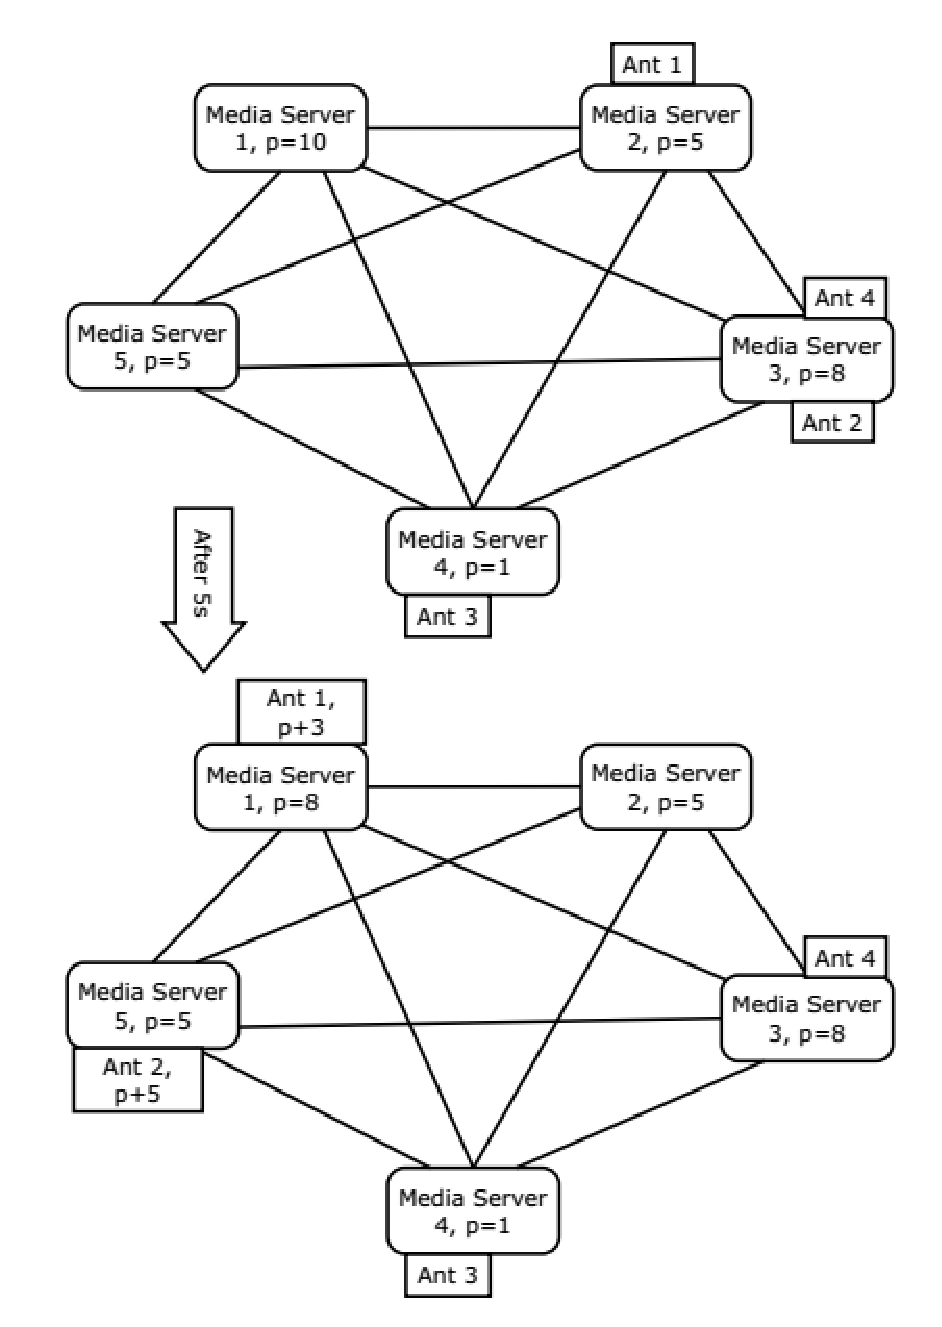
\includegraphics[width=0.9\linewidth]{aco_cloud}
	\caption{Ant Colony Optimization Network}
	\label{fig:antnetwork}
\end{figure}

\subsection{Server and cloud load: Pheromone levels}

For the purpose of controlling the number of servers in the cloud, the pheromone level in the network is used as a proxy for how loaded the entire cloud of servers is and is used to decide when to add or remove servers. As ants move through the network of servers they deposit pheromones - whenever an ant reaches a server it computes how much pheromone to deposit based on the result of the control system for that server. If the server's control system has a result which shows that the server is underloaded then more pheromone is deposited. If the server is overloaded then less pheromone is deposited. At the same time the pheromone amount at each server decays periodically at a constant rate. As such, a large amount of pheromone shows that servers are underloaded and servers should be removed, while a small amount of pheromone shows that servers are overloaded and that servers should be added.

On top of updating the pheromone at each server, each ant is also responsible for measuring the pheromone level at each node it visits. Ants store a history of the last $x$ nodes that they visited and the pheromone level at each of these nodes. Every time an ant moves to a new server, it removes the oldest pheromone value from this list and adds the pheromone at the current node. It then computes an aggregate metric of the pheromone at the last $x$ nodes visited, which is a simple average:

\begin{equation}
p_{ant} = \sum_{i=1}^{N} p_{N} / N
\end{equation}

where $p_{N}$ is the pheromone at server $N$. Once the pheromone level of an ant goes under a predefined value, the ant triggers the algorithm to determine the new count of servers which should be added to the cloud. Similarly, if the pheromone level of an ant becomes too high, the ant triggers the algorithm to determine the number of servers which should be removed from the cloud. The algorithm used to increase or decrease the size of the cloud triggers when more than half of the ants in the system agree that the algorithm should start. Until enough ants agree to start the cloud size optimization the ants continue moving through the network of servers and update the pheromone levels. Once more than half of the ants agree all ants stop and the optimization algorithm starts.

\subsection{Mathematical model}

The pheromone level at a single node is defined base don the previous section as:

\begin{equation}
p^{t}_{n} = p^{t-1}_{n} + \sum_{i=1}^{K}(\tau_{i} * (1 - p)) - \rho
\end{equation}

where $p^{t}_{n}$ is the amount of pheromone at node $n$ at time $t$ where $t$ can be considered discrete in some time increment and $K$ is the amount of ants arriving at the node in the time frame between $t-1$ and $t$.

Based on this equation, there are a number of parameters that can be tuned for the ACO algorithm:

\begin{enumerate}
	\item Decay amount - the amount that the pheromone level decreases at each server: $\rho$
	\item Decay rate - how often does the pheromone level decay at each server: $T_{decay}$
	\item Ant minimum wait time - the minimum wait time for an ant at a server: $T_{minwait}$
	\item Ant pheromone level - the maximum amount of pheromone deposited by an ant at a server: $\tau_{max}$
	\item Ant history size - how many servers an ant should store in it's history
	\item Minimum/maximum trigger level - the minimum/maximum average pheromone level across the last $x$ servers visited by the ant required for the ant to trigger the optimization algorithm: $Pt_{max}$/$Pt_{min}$
\end{enumerate}

Based on these parameters the following three cases can be considered for how the system will behave.

\subsubsection{Under-loaded server}

If an under-loaded server is considered where the ant waits the minimum time and deposits the maximum amount of pheromone and we set $T_{decay} = T_{minwait}$ then in each time period the amount of pheromone at the server can be defined as:

\begin{equation}
\begin{aligned}
p^{t}_{n} &= p^{t-1}_{n} + (\tau_{max} - \rho) \\
p^{t}_{n} &= (n - 1) * (\tau_{max} - \rho)
\end{aligned}
\end{equation}

At the same time the ant will make a decision when $p^{t}_{n} > Pt_{max}$ or $p^{t}_{n} < Pt_{min}$. Because the server is under-loaded we expect that the amount of pheromone will continuously increase since the ant's goal should be to remove servers due to over-provisioning. The ant will make a decision when:

\begin{equation}
\begin{aligned}
p^{t}_{n} &= Pt_{max} \\
(n - 1) * (\tau_{max} - \rho) &= Pt_{max} \\
(n - 1) &= \frac{Pt_{max}}{(\tau_{max} - \rho)} 
\end{aligned}
\end{equation}

As such it can be determined that:

\begin{enumerate}
	\item $\tau_{max}$ must be greater than $\rho$
	\item The time to wait before the ant makes a decision can be defined by $Pt_{max}$ and $(\tau_{max} - \rho)$. A smaller difference between $\tau_{max}$ and $\rho$ will lead to slower decisions, while a smaller $Pt_{max}$ will lead to quicker decisions.
\end{enumerate}

\subsubsection{Balanced server}

If a balanced server is considered - that is a server where the control function shows that the server is well balanced and neither under-loaded, nor overloaded then both the amount of pheromone and the wait time of the ant change. Define $T_{b}$ as the time for the ant to wait at a balanced server and $\tau_{b}$ as the amount of pheromone deposited at a balanced server. Both $T_{b}$ and $\tau_{b}$ are defined in terms of the control function, where $T_{b} = T_{minwait} / (1 - p)$ and $\tau_{b} = \tau_{max} * (1 - p)$

\begin{equation}
\begin{aligned}
p^{t}_{n} &= \frac{t *  \tau_{b}}{T_{b}} - \frac{t *  \rho}{T_{decay}} \\
p^{t}_{n} &= \frac{t *  \tau_{max}(1 - p)}{\frac{T_{minwait}}{1 - p}} - \frac{t *  \rho}{T_{decay}}
\end{aligned}
\end{equation}

The goal of the ant system in such a case is to maintain the level of the pheromone such that servers are not added or removed. As such it can be determined that:

\begin{equation}
\frac{t *  \tau_{max}(1 - p)}{\frac{T_{minwait}}{1 - p}} = \frac{t *  \rho}{T_{decay}}
\end{equation}

which means that the amount of decay equals the amount of pheromone deposited over long periods of time.

\begin{equation}
\begin{aligned}
t *  \tau_{max} * (1 - p) * T_{decay} &= t *  \rho * \frac{T_{minwait}}{1 - p} \\
\tau_{max} * (1 - p)^2 * T_{decay} &= \rho * T_{minwait} \\
\frac{\tau_{max} * (1 - p)^2}{\rho} &= \frac{T_{minwait}}{T_{decay}}
\end{aligned}
\end{equation}

If as in the previous case for an under-loaded server $T_{minwait} = T_{decay}$, then the equation becomes:

\begin{equation}
\begin{aligned}
\tau_{max} * (1 - p)^2 &= \rho
\end{aligned}
\end{equation}

This equation allows the user to set the relation between $\tau_{max}$ and $\rho$ for a given $p$ where the cluster size should be stable. For example, if a cluster size should be stable when $p = 50\%$ then

\begin{equation}
\begin{aligned}
\tau_{max} * (0.5)^2 &= \rho \\
\tau_{max} * 0.25 &= \rho
\end{aligned}
\end{equation}

\subsubsection{Over-loaded server}

The previous equation holds for an over-loaded server as well. If we take the same example as before where the system is set to be balanced for $p = 50\%$, if $p$ goes up to $90\%$ then the previous equation becomes:

\begin{equation}
\begin{aligned}
p^{t}_{n} &= \frac{t *  \frac{\rho}{0.25} * 0.1}{\frac{T_{decay}}{0.1}} - \frac{t *  \rho}{T_{decay}} \\
p^{t}_{n} &= \frac{t *  \frac{\rho}{0.25} * 0.1}{\frac{T_{decay}}{0.1}} - \frac{t *  \rho}{T_{decay}} \\
p^{t}_{n} &= \frac{t * \rho}{T_{decay}} * (0.04 - 1) \\
p^{t}_{n} &= \frac{t * \rho}{T_{decay}} * -0.96
\end{aligned}
\end{equation}

This equation means that the pheromone rate at the node will decrease by $\rho * -0.96$ every decay period.

Once enough of the ants discover that either the minimum or maximum threshold is breached, the cloud size optimization self-organizing algorithm triggers.

\subsection{Cloud size optimization: Ant house hunting}

The ant house hunting algorithm is inspired by the behaviour ant colonies use in order to reach consensus decisions in the case of relocating the nest as in \cite{selforg:antreloc} and \cite{selforg:antreloc2}. Ants use a complex, distributed approach to find a new nest which involves some ants searching for a new nest, scout ants communicating with each other about the suitability of a discovered nest, recruitment of other scout ants to a discovered nest, and finally a majority of ants agreeing on a new nest and moving the ant colony to the new nest.

Initially, when the nest is in danger of being destroyed ants start searching for a new nest where the colony can relocate. In this phase, scouting ants leave the nest and search for a new location for the colony to relocate to. Once a scout finds a suitable location, it evaluates the location based on various factors and then returns to the home nest. Once a scout ant is satisfied with the new nest it goes back to the home nest and starts recruiting other ants to its chosen nest. Ants then start doing tandem runs where one ant leads another. Upon arriving at a new nest, a recruited ant evaluates the new nest and then starts doing tandem runs if the new nest is acceptable. At this point there are many possible nests and the ants must reach a consensus as to which nest will be the new home. One approach that ants are assumed to use is that of quorum threshold \cite{selforg:ant-quorum}. When ants reach the home nest they check if a quorum has been reached and if yes, they start to move the entire ant colony to the new nest.

\subsection{Model for Cloud size optimization}

Based on the above natural process, a self-organizing system can be developed in order to optimize the number of servers in the cloud by having an ant colony search for the optimal number of servers which should be up in the cloud at a given time. This algorithm works by having each ant in the ant colony search for a new nest, where a nest is represented by a new optimum number of servers in the cloud. The ants are the same ants for the ACO algorithm. When the SLA breach is predicted the ants morph to house hunting ants and start to look for a new home. The algorithm assumes that there is a home nest where the ants can meet after searching for a new nest and exchange information. Once all the ants have agreed on the same optimum value, the servers are added or removed as desired and all ants are morphed back into food foraging ants for the ACO algorithm.

The model for optimizing the size of the cloud is composed of three components:

\begin{enumerate}
	\item Nest candidates - each nest candidate represents a possible solution in term of the number of servers that should be up in the server
	\item House hunting ants - ants are simple agents which search for a new home nest
	\item Mathematical model - this is the model which represents the viability of a nest from the point of view of an ant.
\end{enumerate}

\subsection{Nest candidates}

For each ant that morphs into a house hunting ant a new nest is created. The nest is initialized with a value representing the number of servers which should be up in the cloud if the nest is selected as the new home. These possible solutions are computed as permutations of the current size of the cloud as known by ant which will have the nest as its first candidate. If the ant was morphed because of lack of pheromone, then a random value is generated which represents the number of servers to be added. Each random value is proportional to the size of the cloud and the pheromone level across the last $N$ servers known by the ant. For example, if the cloud contains 100 servers, then the ant would be initialized with a random values, which is defined as:

\begin{equation}
ServerCount_{add} = \frac{N}{2} * rand + \frac{N}{2} * \frac{Pt_{max} - p_{ant}}{Pt_{max}}
\end{equation}

where $rand$ is a random value between 0 and 1 and $p_{ant}$ is the average pheromone level seen by the ant across the last $n$ servers it went to. The pheromone is used as a scaling factor such that the lower the pheromone value, the higher the probability of more servers being added. The random value has the effect of generating multiple possible solutions across different ants.

If however the ant was morphed because of too much pheromone, then the nest does a similar initialization where it computes the number of servers to remove as:

\begin{equation}
ServerCount_{remove} = \frac{N}{2} * rand + \frac{N}{2} * \frac{p_{ant} - Pt_{max}}{Pt_{max}}
\end{equation}

Similar to the add case, the higher the pheromone level compared to the maximum threshold the more servers will be removed from the cloud.

\subsection{Self-organizing agent: House hunting ant}

In order for an ant to determine the viability of a nest, the ant will check the number of servers to add or remove and simulate what effect that will have on the ants pheromone levels. If the cloud should increase in size, then the ant replaces a proportional number of servers in its history with empty servers and then recalculate the average pheromone across those servers. If the cloud should decrease in size, then the ant removes a proportional number of servers in its history and then redistributes the pheromone across the remaining servers.

For example, if the ant has in its history 10 servers and the nest has a desired server value of 15, then the ant will hide 3 of its servers and replace them with 3 servers with medium pheromone level and recalculate the average pheromone across the servers. If however the ant has in its history 10 servers and the nest has a desired server value of 7, then the ant will hide 3 of its servers and redistribute the pheromone from those 3 servers on the remaining 7 levels.

The house hunting algorithm is performed in rounds and ants can be in one of four states:

\begin{enumerate}
	\item Search - This is the initial state of ants which search for a new nest
	\item Active - The ant is committed to a good nest and tries to recruit other ants to it
	\item Passive - The ant is committed to a bad nest and is waiting to be recruited
	\item Final - A single nest remains so all ants go to it and that is the solution
\end{enumerate}

The state diagram for the ants can be described as in Figure \ref{fig:anthousehuntingstate}

\begin{figure}
	\centering
	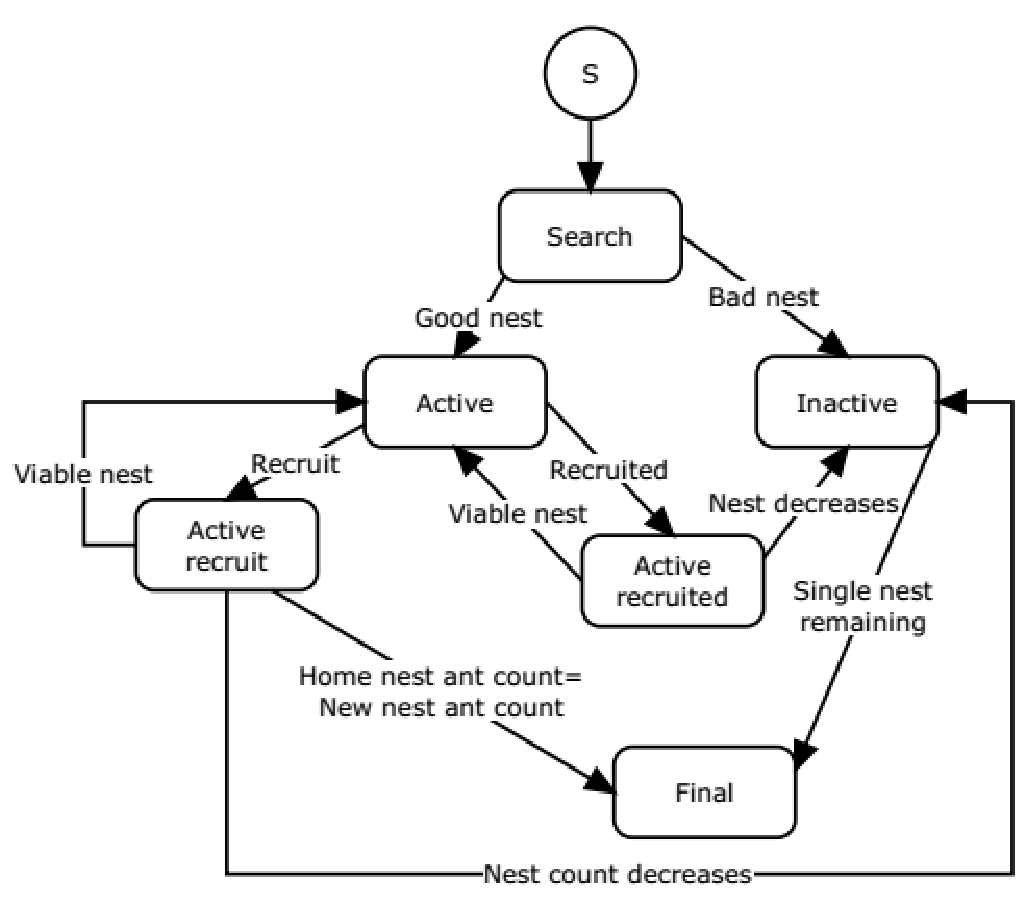
\includegraphics[width=0.9\linewidth]{aco_state}
	\caption{Ant House Hunting State Diagram}
	\label{fig:anthousehuntingstate}
\end{figure}

In the first round all house hunting ants initialize a nest and go to it. The ants then simulate the performance of the solution as described previously. If the simulated result's performance is under a given threshold, then the ant goes into the passive state, otherwise it goes into the active state.

In the second round, all ants return to the home nest and active ants try to recruit other ants at the home nest. Passive ants can not be recruited until the final round when all ants go to the single remaining nest. Active ants recruit randomly from the other active ants at the home nest by choosing another ant to recruit and bring it to it's committed nest. In order to ensure no conflicts between recruiting ants, the ants recruit iteratively and an ant which was already recruited does not recruit someone else. This recruitment is biased by the perceived suitability of the nest by the ants, such that better nests are given priority. The bias is achieved by sorting the ants by the perceived viability and then randomly choosing a recruiter ant such that ants with better suitability have a higher chance of being recruiters and ants with lower viability have a higher chance of being recruited. This is achieved using the following formula, where the probability of an ant to recruit is defined as the viability of the ant's chosen nest divided by the sum of all the ant's chosen nests.

\begin{equation}
p_{recruit} = ant_{viability} / \sum\limits_{i=1}^n ant_{viability}
\end{equation}

Once an ants recruits another ant the two ants go together to the nest of the recruiting ant. When reaching a new nest, active ants count the number of ants at the nest and check if the nest they reached is the same as the previous nest they went to. Based on the number of ants and the nest there are three cases:

\begin{enumerate}
	\item If the nest is the same nest that the ant went to before and the number of ants has increased or remained the same then the nest is still a possible solution so the ant updates the count and waits an extra round at the nest. After waiting a round, the ant checks if the number of ants at the home nest is the same as that at its current nest. If they are the same then the ant goes to the final state, new servers are added or removed and all ants morph back to ACO ants.
	\item If the nest is the same nest that the ant went to before and the number of ants has decreased then the ant becomes passive because the nest is in the process of being dropped out. The ant returns home in the same round that active ants wait at the new nest.
	\item If the nest is different then the nest the ant was committed to then the ant waits a round and then it checks to see if the number of ants at its new nest has decreased or not. If the number has decreased, then this nest is dropping out as the ants already committed to it have gone to the home nest and the ant becomes passive. Otherwise, the ant commits to its new nest and goes home to recruit other ants.
\end{enumerate}

The above algorithm can be described as follows in pseudo-code in Figure \ref{ant:pseudocodeHouseHunting}. $R_{x}$ represents round x.

\begin{algorithm}
\begin{algorithmic}
	\State $R_{1}$: Go to new nest
	\State Compute suitability of new nest
	\If{Suitability $<$ threshold}
		Switch to passive
	\EndIf
	\State $R_{2}$: Go to home nest
	\If{Ant is active \&\& Ant is not recruited}
		\State Recruit another ant
		\State Go to new nest
	\ElsIf{Ant is recruited}
		\State Go to new nest
	\EndIf
	\State $R_{3}$: Count number of ants at new nest = $count_{new}$
	\If{Nest is same and $count_{new} >= count_{old}$}
		\State Wait round
	\ElsIf{Nest is same and $count_{new} < count_{old}$}
		\State Switch to passive
		\State Go to home nest
	\ElsIf{Nest is different}
		\State Wait round
	\EndIf
	\State $R_{4}$: Count number of ants at new nest $count_{new}$
	\If{$count_{new} == count_{home}$}
		\State Switch to final state
	\ElsIf{$count_{new} < count_{old}$}
		\State Switch to passive
		\State Go to $R_{2}$
	\EndIf
	\State Return final state
	\State Switch ants to ACO ants
\end{algorithmic}
\caption{Ant House Hunting Pseudocode}\label{ant:pseudocodeHouseHunting}
\end{algorithm}

\subsection{Mathematical model: nest viability}

In order to determine if a nest should be considered as a solution ants must determine the viability of the nest. Because it is impossible for ants to predict how the user requests would be processed by more/less servers the ants use a heuristic to approximate the viability of each solution. It is important to note that due to each ant having a different memory of servers it has recently visited, different ants will see the same nest as having a different viability score.

There are two cases to consider - one when a cloud is over-loaded and servers should be added, and one where the cloud is under-loaded and servers should be removed.

\subsubsection{Over-loaded cloud}

In the case of an over-loaded cloud, each of the nests will have its solution contain more servers than the count of servers known by each ant. As such in order to determine the viability of the nest, the ant needs to simulate how a cloud with the extra servers would behave. The ant only has a short memory of its last $x$ visited servers and the amount of pheromone at these servers when it visited them. Because of this, the ant assumes that it would have visited the new servers with equal probability, so it replaces $y$ servers in its history with servers with optimal pheromone level, where the optimal pheromone level is defined as:

\begin{equation}
	p_{opt} = \frac{Pt_{max} + Pt_{min}}{2}
\end{equation}

and 

\begin{equation}
	y = x * \frac{newServerCount - cloudSize}{newServerCount}
\end{equation}

As such, the ant computes the average pheromone level across the last $x$ servers it would have visited as:

\begin{equation}
	p_{averageScaled} = \frac{y * p_{opt} + \sum\limits_{i=y+1}^x p_{i}}{x}
\end{equation}

Finally, the viability of the nest is defined as:

\begin{equation}
	viability = 1 - \frac{\left|p_{averageScaled} - p_{opt}\right|}{p_{opt}}
\end{equation}

With this approach, the ant simulates how the system would behave if it had $y$ extra servers taking some of the load from the existing servers. It then computes the viability based on how close the simulated pheromone is to the optimal pheromone.

\subsubsection{Under-loaded cloud}

In the case of an under-loaded cloud, each of the nests will have its solution contain less servers than the count of servers known by each ant. As such in order to determine the viability of the nest, the ant needs to simulate how a cloud with the lower count of servers would behave. The ant computes a number of servers $y$ in its history which should be removed as:

\begin{equation}
	y = x * \frac{cloudSize - newServerCount}{cloudSize}
\end{equation}

and then simulates the average pheromone for the cloud as:

\begin{equation}
	p_{averageScaled} = \frac{\sum\limits_{i=y+1}^x p_{i}}{x}
\end{equation}

The viability of the nest is calculated as in the case of the overloaded cloud. With this approach, the ant simulates how the system would behave if it had $y$ less servers and the remaining servers are taking the load from the removed servers. The viability is computed based on how close the simulated pheromone is to the optimal pheromone.

\section{Simulation Environment}
\label{sec:testbed}

In order to test the performance of the self-organizing system previously described, a simulation was created on top of the CloudSim and CloudSimEx systems. CloudSim is a framework for modelling and simulating cloud systems in which various tests can be run - for example the placement of tasks in a cloud or the performance of a cloud system. CloudSim allows users to define datacenters which are composed of hosts which can run virtual machines and virtual machines which run on top of the hosts. Both hosts and virtual machines are defined in terms of million instructions per second (MIPS) and memory available. Once a datacenter is defined, a workload can be defined as well to be executed in the datacenter. CloudSim workloads are called cloudlets - a cloudlet represents a user task and defines how many million instructions (MI) the task takes as well as how much memory the task needs. As such a cloudlet's execution time will depend on its' lifetime in MIs and how many MIPS the VM the cloudlet is allocated to has. The usage of MIPS and MI to represent loads and available resources make it complicated to define workloads that would represent real world behaviours.

CloudSimEx extends CloudSim by adding the concept of web sessions. Internally a web session is composed of a number of web cloudlets, where each web cloudlet has a small RAM and MIPS requirements and later web cloudlets in a web session can not be completed until all previous web cloudlets have completed. Web sessions also have the property of targeting both application server VMs and database VMs, with the web session alternating cloudlets running on either application server or database server. Furthermore, CloudSimEx also adds the concept of scaling policies which can be applied on a cloud. A scaling policy adds or removes servers to/from the cloud when the policy determines that some conditions are breached. A basic policy is implemented in CloudSimEx which scales the cloud when the CPU usage passes certain thresholds and also includes a quiet time after a scaling action has been performed. The basic policy implements an interface which makes it easy to add other scaling policies. 

Because CloudSim and CloudSimEx only include CPU usage and memory usage as measurable metrics, the simulation of the self-organizing system uses the CPU usage as an input for the ACO algorithm to determine how the pheromone should be updated. In order to run the self-organizing system in this paper and compare it to existing results, a number of workloads which are predefined in CloudSimEx are used.

The architecture of the simulation framework is presented in Figure \ref{fig:simulation-design}.

\begin{figure}
	\centering
	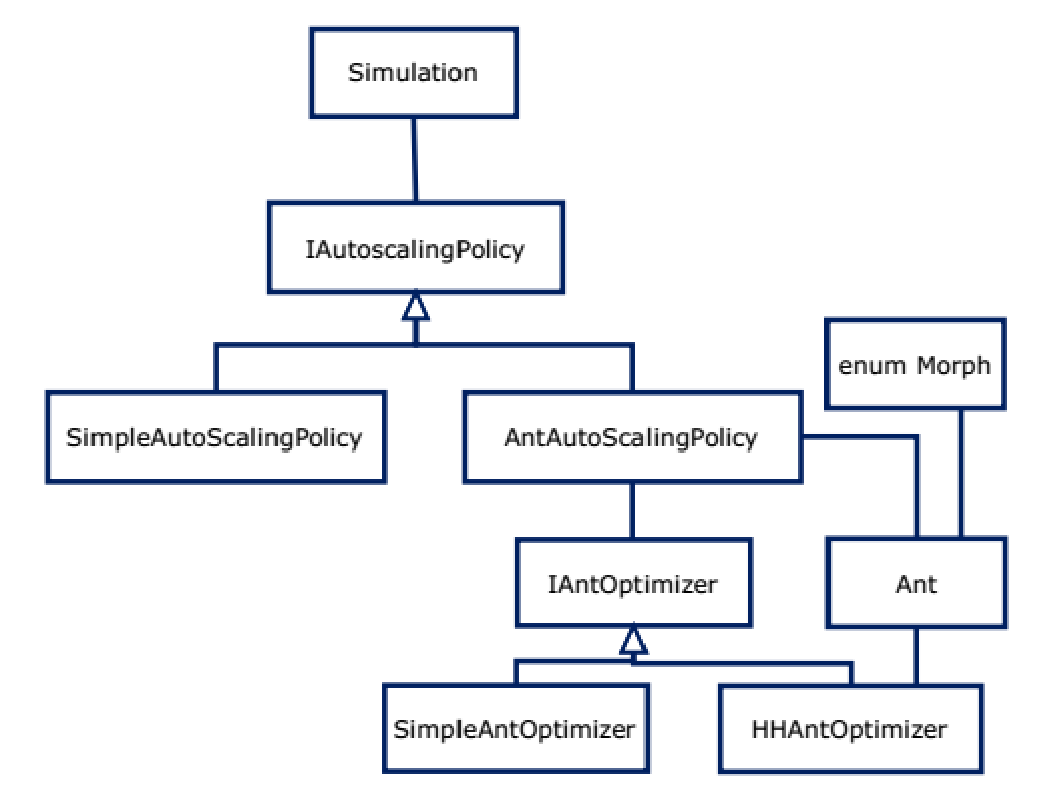
\includegraphics[width=0.9\linewidth]{simulation_archi}
	\caption{Simulation Framework System}
	\label{fig:simulation-design}
\end{figure}

The simulation runs three different scaling policies for comparison. The first scaling policy used is the simple scaling policy provided by CloudSimEx. This scaling policy measures the average CPU usage of the cloud and when predefined thresholds are breached it either adds one server if the upper threshold is breached or removes one server if the lower threshold is breached. The policy also includes a quiet time, which is a period of time after an action was taken during which no other action will be taken. For the purpose of these tests the thresholds for the simple scaling policy are set to:

\begin{description}
	\item[Upper threshold] is set to 80\% average CPU utilization across the cloud
	\item[Lower threshold] is set to 10\% average CPU utilization across the cloud
	\item[Quiet time] is set to 150s during which no other action will be taken
\end{description}

The values chosen match the default values for the Amazon EC2 auto scaling policy.

The second policy is based on the predictive ACO algorithm presented in this paper but without the house hunting algorithm to determine the number of instances to scale up or down. The policy uses the ACO algorithm to determine when instances should be added or removed. When a decision is taken that servers need to be added or removed a single server instance is added or removed at one time. The ACO policy does not need quiet time defined as it inherently includes quiet time due to the fact that it takes time for the pheromone to build up or decrease. For the purpose of these simulations the ACO algorithm runs with the following parameters:

\begin{description}
	\item[Decay amount] is set to 1
	\item[Decay period] is set to 15s
	\item[Minimum ant wait time at an under-loaded node] is set to 1s
	\item[Maximum ant pheromone added at an under-loaded node] is set to 4
	\item[Ant memory size] is set to 5
	\item[Pheromone level for triggering server removal] is set to 100
	\item[Pheromone level for triggering server addition] is set to 25
	\item[CPU is considered to be balanced] if it is between 45\% and 55\% utilization
\end{description}

The third tested policy contains both the ACO algorithm for prediction of SLA breaches and the house hunting algorithm for the optimization of the cloud size when a breach is detected. The tests are run with the same parameters as the second policy.

\section{Results}
\label{sec:results}

The performance of the self-organizing system presented in this paper was run on top of the simulation environment presented in the previous section. A number of tests were run, with different workloads in order to determine the performance of the system and also compare how the developed ant based system performs compare to other auto scaling systems. Due to the fact that the workloads are generated stochastically, each of the tests was run 5 times and the results were aggregated. The performance tests only focus on the auto-scaling algorithm for the application tier and assume that the cloud has enough hosts and also that the cloud has enough database VMs to take care of the load. For this purpose all simulations are run with 60 host computers which can run VMs and 30 database VMs which are always up. Each of the hosts is defined as having 2 CPU cores, each of which provides 1000 MIPS. All of the application VMs are equal in power and they provide 250 MIPS to the simulated web application running on top of the VM. Each of the simulations is run for 48 hours, with a workload defined for 24 hours and which repeats after the first 24 hours. Workloads are generated using a Gaussian distribution.

\subsection{Low workload, low number of VMs}

The first simulation run is a simulation where the workload is low and as such not a large number of VMs are required to run at the same time in order to meet the desired SLAs for the application.

The workload for this test starts with a mean of 60 sessions per hour and a standard deviation of 1 and gradually increases towards a mean of 1000 sessions per hour with a standard deviation of 5, at 10 - 12 hours. This is followed by a small drop at 13 hours to 500 sessions after which the load goes back to 1000 sessions for hour until 17 hours. After this, the workload decreases gradually until it reaches 30 sessions per hour with a standard deviation of 1 at 24 hours. The distribution of the sessions per hour can be seen in Figure \ref{fig:sim1-workload}. This test simulates a usual workload seen in online services where the demand peaks at one point during the day.

\begin{figure}
	\centering
		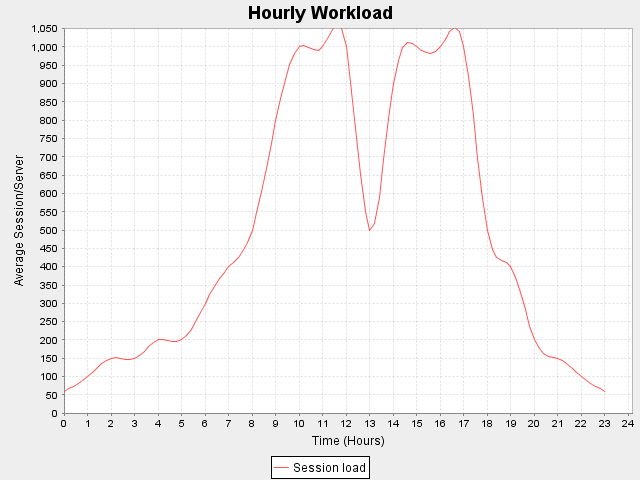
\includegraphics[width=0.75\columnwidth]{results/sim1/sim1-workload.png}
	\caption{Simulation - low workload}
	\label{fig:sim1-workload}
\end{figure}

Figures \ref{fig:sim1-basestats}, \ref{fig:sim1-antSimplestats} and \ref{fig:sim1-antHHstats} show the statistical results for the simulation runs. The results are averaged per hour and across the 5 runs for each auto-scaling algorithm. The graphs include average CPU usage as well as average number of sessions per server and average provisioned servers. Looking at the three graphs, it can be seen that the simple ant auto scaling algorithm obtains better CPU utilization than the simple auto scaling approach, and better than the house hunting algorithm also. At the same time, the simple ant auto scaling algorithm achieves this, while maintaining the server count more stable than the simple auto scaling algorithm.

\begin{figure}
	\centering
		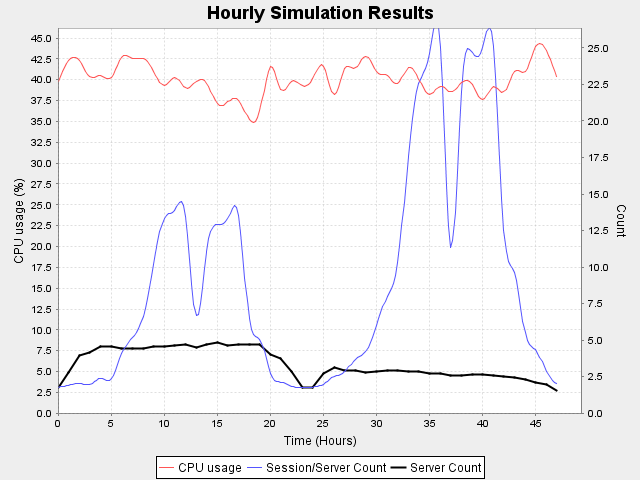
\includegraphics[width=0.75\columnwidth]{results/sim1/sim1-basestats.png}
	\caption{Simulation - Low workload: Simple autoscaling}
	\label{fig:sim1-basestats}
\end{figure}

\begin{figure}
	\centering
		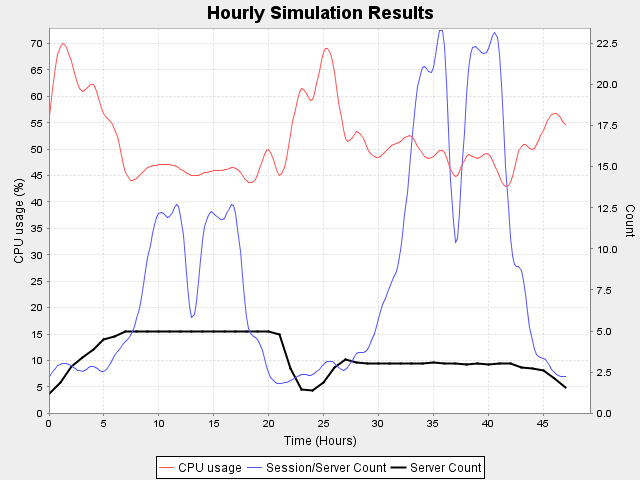
\includegraphics[width=0.75\columnwidth]{results/sim1/sim1-antSimplestats.png}
	\caption{Simulation - Low workload: Simple ant autoscaling}
	\label{fig:sim1-antSimplestats}
\end{figure}

\begin{figure}
	\centering
		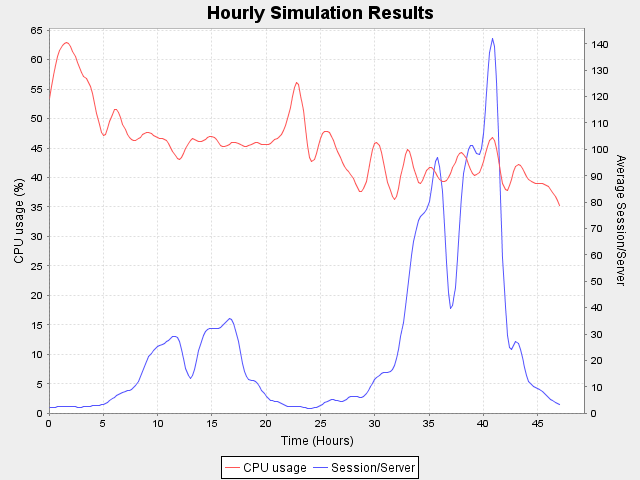
\includegraphics[width=0.75\columnwidth]{results/sim1/sim1-antHHstats.png}
	\caption{Simulation - Low workload: House hunting ant autoscaling}
	\label{fig:sim1-antHHstats}
\end{figure}

Similar results can be seen in Table \ref{table:sim1} which summarizes the tests. Scale up and scale down count represents the number of times the optimizer decided to add or remove servers. A decision to add N servers, counts as a single scale up action. $Over provisioned - x\%$ represents the time in seconds that the average utilization of the cloud was under $x\%$, suggesting low utilization and over provisioning of the cloud. Similarly $High usage - x\%$ represents the time in seconds that the utilization of the cloud was over $x\%$. This could be either due to under provisioning if response times are delayed at the same time, or can be a sign of good provisioning if sessions still end fine. $Average session delay$ represents the average delay across all of the sessions, while $Max session delay$ represents the maximum delay. CloudSim defines a desired end time for a session, which represents when the session should end if there are no delays due to scheduling. Delay is defined as the time it took for the session to complete after this desired end time.

The simple scaling algorithm takes a lot more scale up and scale down actions than the two ant based algorithms. This is because as soon as the average utilization breaches the thresholds an action must be taken, while for the ant algorithms the detection is not triggered by a single drop or spike in utilization. At the same time, the simple ant scaling algorithm has a much shorter time when the cloud is over provisioned (too many servers for the load) compared to the simple scaling algorithm, and longer periods when the cloud is under high usage with over 70\% and 80\% CPU usage. The house hunting algorithm performs worse than the simple ant algorithm for this test, as it tends to over provision the cloud when a breach is predicted by adding too many servers. This can be seen, as it has higher scale up/down counts and also higher over provisioned times. The delay results in table \ref{table:sim1-delay} show similar behaviour with the simple ant algorithm behaving better than the simple scaling algorithm and the house hunting algorithm behaving worse.

\begin{table}
\caption{Low workload simulation results - utilization}
\label{table:sim1}
\begin{tabu} to\linewidth{|X[c]|X[c]|X[c]|X[c]|X[c]|X[c]|X[c]|}
\everyrow{\hline}
\hline
Scaling Algorithm & Scale Up Count & Scale Down Count & Over Provisioned - 20\% (s) & Over Provisioned - 40\% (s) & High usage - 70\% (s) & High usage - 80\% (s) \\
\taburowcolors 2{Gray!20..LimeGreen!50}
Simple scaling & 755 & 762 & 7140 & 88423 & 3048 & 1080 \\
Simple ant scaling & 128 & 132 & 2796 & 40104 & 16008 & 7260 \\
House hunting scaling & 223 & 339 & 16656 & 53352 & 11184 & 5904 \\
\end{tabu}
\end{table}

\begin{table}
\caption{Low workload simulation results - delays}
\label{table:sim1-delay}
\begin{tabu} to\linewidth{|X[c]|X[c]|X[c]|X[c]|}
\everyrow{\hline}
\hline
Scaling Algorithm & Average Delay (s) & Maximum delay & Average Servers  \\
\taburowcolors 2{Gray!20..LimeGreen!50}
Simple scaling & 28.8 & 118.6 & 3.35 \\
Simple ant scaling & 20.5 & 75.3 & 3.49 \\
House hunting scaling & 115.4 & 574.3 & 1.95 \\
\end{tabu}
\end{table}

\subsection{High workload, high number of VMs}

The second test uses the same workload as the first test but scaled 5 times. With this scaling the simulation ends up requiring a large number of servers. The distribution of the sessions per hour can be seen in Figure \ref{fig:sim2-workload}.

Figures \ref{fig:sim2-basestats}, \ref{fig:sim2-antSimplestats} and \ref{fig:sim2-antHHstats} show the statistical results for the simulation runs. The results are averaged per hour and across the 5 runs for each auto-scaling algorithm. Looking at the three graphs, it can be seen that the simple ant auto scaling algorithm and the simple auto scaling approach behave very similar. Both increase the number of servers as demand increases, and then once demand decreases they both decrease the number of servers in the cloud. Due to the fact that the two algorithms add servers one by one, they end up under provisioning the cloud when demand is high and over provisioning when demand goes low. The house hunting algorithm behaves much better than the two simple scaling algorithms as it is able to keep up with the demand by adding more servers at one time and removing more servers at the same time. The same results can be seen in Table \ref{table:sim2}. The house hunting algorithm is able to achieve better server utilization - only 768 seconds of average CPU utilization under 20\% compared to more than 20000s for the simple scaling algorithms, while performing less scale up/scale down actions. The delay results in table \ref{table:sim2-delay} are very similar for all 3 scaling algorithms with average delay at, or near 0 and very small maximum delays. In such a case, the house hunting algorithm behaves better as it takes less actions and uses less servers than the simple scaling algorithm.

\begin{figure}
	\centering
		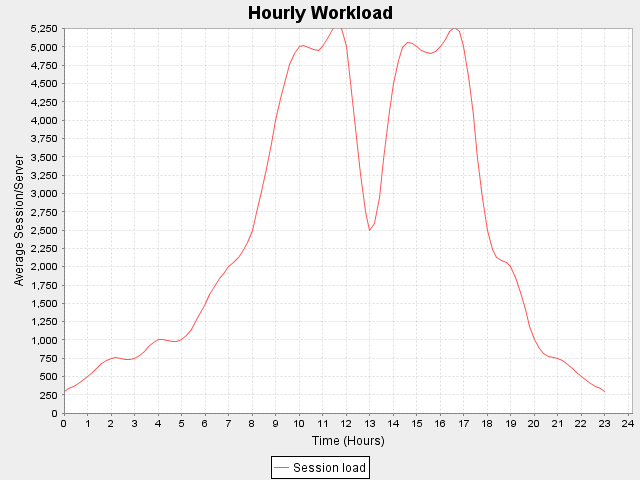
\includegraphics[width=0.75\columnwidth]{results/sim2/sim2-workload.png}
	\caption{Simulation - High workload}
	\label{fig:sim2-workload}
\end{figure}

\begin{figure}
	\centering
		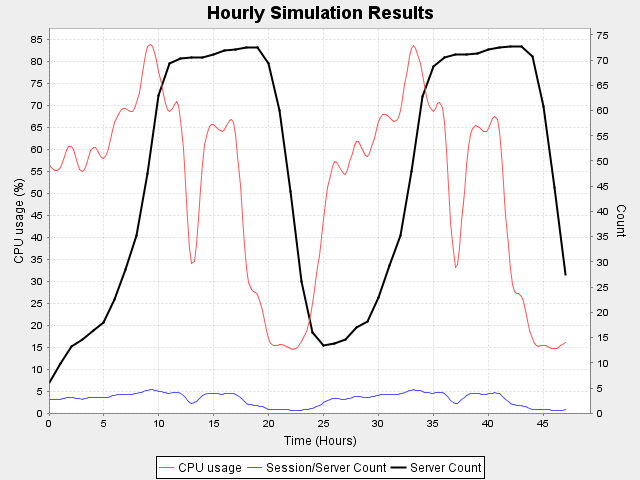
\includegraphics[width=0.75\columnwidth]{results/sim2/sim2-basestats.png}
	\caption{Simulation - High workload: Simple autoscaling}
	\label{fig:sim2-basestats}
\end{figure}

\begin{figure}
	\centering
		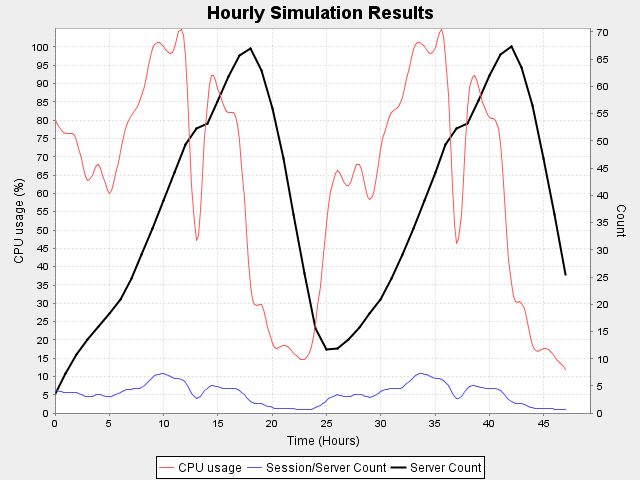
\includegraphics[width=0.75\columnwidth]{results/sim2/sim2-antSimplestats.png}
	\caption{Simulation - High workload: Simple ant autoscaling}
	\label{fig:sim2-antSimplestats}
\end{figure}

\begin{figure}
	\centering
		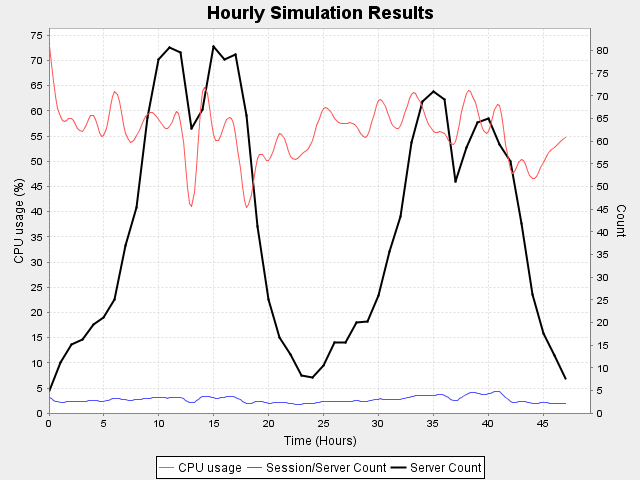
\includegraphics[width=0.75\columnwidth]{results/sim2/sim2-antHHstats.png}
	\caption{Simulation - High workload: House hunting ant autoscaling}
	\label{fig:sim2-antHHstats}
\end{figure}

\begin{table}
\caption{High workload simulation results}
\label{table:sim2}
\begin{tabu} to\linewidth{|X[c]|X[c]|X[c]|X[c]|X[c]|X[c]|X[c]|}
\everyrow{\hline}
\hline
Scaling Algorithm & Scale Up Count & Scale Down Count & Over Provisioned - 20\% (s) & Over Provisioned - 40\% (s) & High usage - 70\% (s) & High usage - 80\% (s) \\
\taburowcolors 2{Gray!20..LimeGreen!50}
Simple scaling & 717 & 693 & 26255 & 50503 & 8952 & 231 \\
Simple ant scaling & 661 & 656 & 22241 & 42750 & 85873 & 62593 \\
House hunting scaling & 332 & 253 & 768 & 32643 & 35419 & 18631 \\
\end{tabu}
\end{table}

\begin{table}
\caption{High workload simulation results - delays}
\label{table:sim2-delay}
\begin{tabu} to\linewidth{|X[c]|X[c]|X[c]|X[c]|}
\everyrow{\hline}
\hline
Scaling Algorithm & Average Delay (s) & Maximum delay & Average Servers  \\
\taburowcolors 2{Gray!20..LimeGreen!50}
Simple scaling & 0 & 14.1 & 46.9 \\
Simple ant scaling & 1.1 & 15.3 & 37.7 \\
House hunting scaling & 1.1 & 28.4 & 40.9 \\
\end{tabu}
\end{table}

\subsection{Very high workload, very high number of VMs}

The final test uses a very high workload with an initial peak of 5000 sessions/hour after 5 hours, followed by a decrease in requests and a second much higher peak of 10000 sessions/hour after 12 hours. The distribution of the sessions per hour can be seen in Figure \ref{fig:sim3-workload}.

Figures \ref{fig:sim3-basestats}, \ref{fig:sim3-antSimplestats} and \ref{fig:sim3-antHHstats} show the statistical results for the simulation runs. The results are averaged per hour and across the 5 runs for each auto-scaling algorithm. Looking at the three graphs, the house hunting algorithm again performs the best, however the simple ant autoscaling algorithm performs worse than the simple autoscaling algorithm. Both simple autoscaling algorithms have trouble as the demand increases quickly, but the simple ant autoscaling can not answer quickly enough. This is due to the fact that there's a certain time needed for the pheromones to pass the trigger level, and after the trigger is passed only a single server can be added. This results in long periods when all the servers are overloaded and average CPU usage is 100\%. Compared to the two simple autoscaling algorithms, the house hunting algorithm behaves much better reaching the optimal number of servers quicker and maintaining this number of servers.

The same results can be seen in Table \ref{table:sim3}. The house hunting algorithm is able to achieve better server utilization again - only 2000 seconds of average CPU utilization under 20\% compared to more than 15000 and 46000s for the two simple scaling algorithms, while performing less scale up/scale down actions.  The delay results in table \ref{table:sim3-delay} show the house hunting algorithm with slightly higher average delays than the other two algorithms, and much higher maximum delay. This can be explained by the fact that the other two algorithms overprovision - seen by the over provision metrics, while the house hunting algorithm underprovisions in a worst case.

\begin{figure}
	\centering
		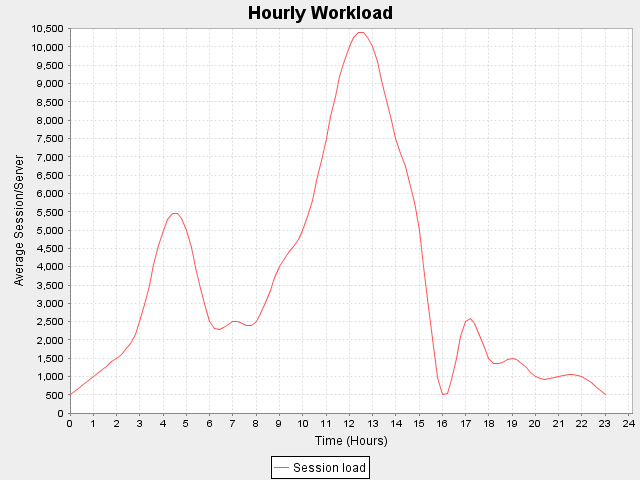
\includegraphics[width=0.75\columnwidth]{results/sim3/sim3-workload.png}
	\caption{Simulation - very high workload}
	\label{fig:sim3-workload}
\end{figure}

\begin{figure}
	\centering
		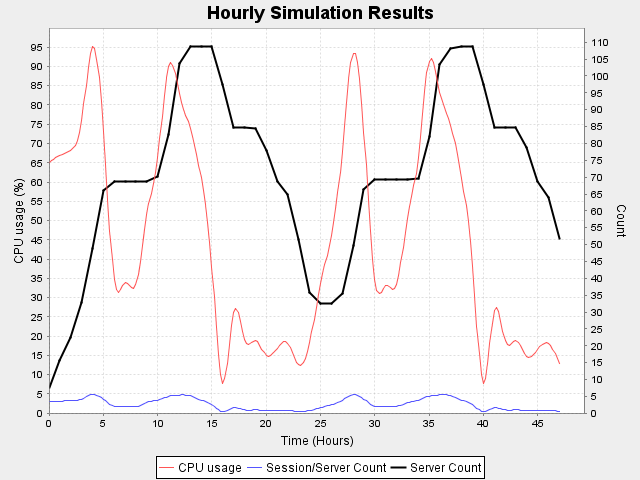
\includegraphics[width=0.75\columnwidth]{results/sim3/sim3-basestats.png}
	\caption{Simulation - Very high workload: Simple autoscaling}
	\label{fig:sim3-basestats}
\end{figure}

\begin{figure}
	\centering
		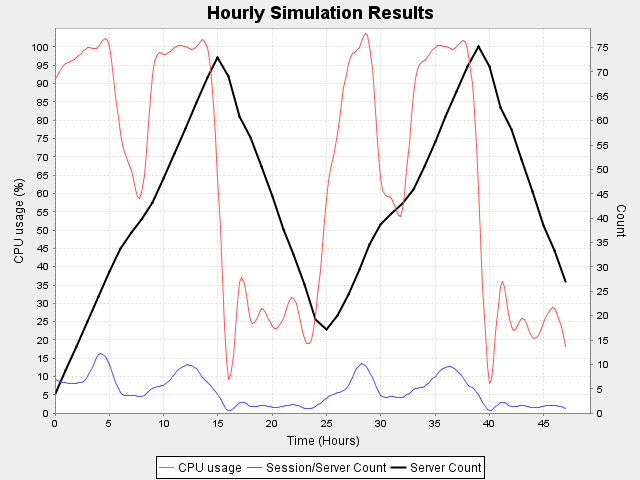
\includegraphics[width=0.75\columnwidth]{results/sim3/sim3-antSimplestats.png}
	\caption{Simulation - Very high workload: Simple ant autoscaling}
	\label{fig:sim3-antSimplestats}
\end{figure}

\begin{figure}
	\centering
		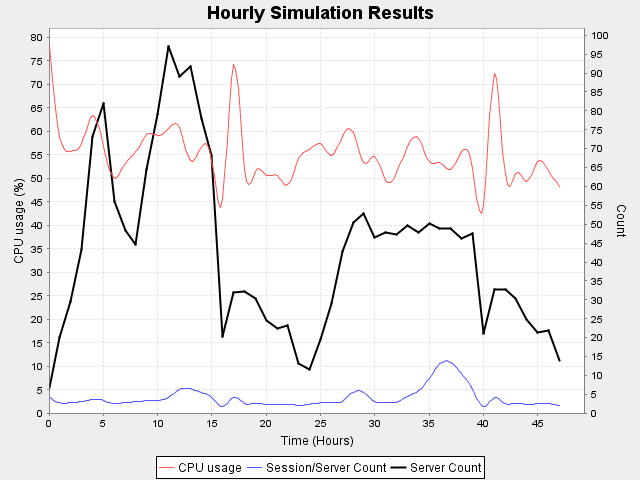
\includegraphics[width=0.75\columnwidth]{results/sim3/sim3-antHHstats.png}
	\caption{Simulation - Very high workload: House hunting ant autoscaling}
	\label{fig:sim3-antHHstats}
\end{figure}

\begin{table}
\caption{Very high workload simulation results}
\label{table:sim3}
\begin{tabu} to\linewidth{|X[c]|X[c]|X[c]|X[c]|X[c]|X[c]|X[c]|}
\everyrow{\hline}
\hline
Scaling Algorithm & Scale Up Count & Scale Down Count & Over Provisioned - 20\% (s) & Over Provisioned - 40\% (s) & High usage - 70\% (s) & High usage - 80\% (s) \\
\taburowcolors 2{Gray!20..LimeGreen!50}
Simple scaling & 1004 & 833 & 46339 & 86035 & 42768 & 20604 \\
Simple ant scaling & 726 & 679 & 16412 & 54641 & 83245 & 76837 \\
House hunting scaling & 354 & 287 & 1956 & 33864 & 32151 & 22080 \\
\end{tabu}
\end{table}

\begin{table}
\caption{High workload simulation results - delays}
\label{table:sim3-delay}
\begin{tabu} to\linewidth{|X[c]|X[c]|X[c]|X[c]|}
\everyrow{\hline}
\hline
Scaling Algorithm & Average Delay (s) & Maximum delay & Average Servers  \\
\taburowcolors 2{Gray!20..LimeGreen!50}
Simple scaling & 1 & 27.6 & 70.6 \\
Simple ant scaling & 3.9 & 22.5 & 43.2 \\
House hunting scaling & 10.7 & 192 & 42.8 \\
\end{tabu}
\end{table}

The performance tests show that the system behaves as desired and that the ACO algorithm properly detects a breach of SLA when the cloud is under loaded or over loaded while the house hunting algorithm can determine the number of servers added or removed. Due to the randomness which exists inside the house hunting algorithm it is possible to overshoot or undershoot the correct number of servers, however this is corrected quickly after another SLA breach is detected.

% An example of a floating figure using the graphicx package.
% Note that \label must occur AFTER (or within) \caption.
% For figures, \caption should occur after the \includegraphics.
% Note that IEEEtran v1.7 and later has special internal code that
% is designed to preserve the operation of \label within \caption
% even when the captionsoff option is in effect. However, because
% of issues like this, it may be the safest practice to put all your
% \label just after \caption rather than within \caption{}.
%
% Reminder: the "draftcls" or "draftclsnofoot", not "draft", class
% option should be used if it is desired that the figures are to be
% displayed while in draft mode.
%
%\begin{figure}[!t]
%\centering
%\includegraphics[width=2.5in]{myfigure}
% where an .eps filename suffix will be assumed under latex, 
% and a .pdf suffix will be assumed for pdflatex; or what has been declared
% via \DeclareGraphicsExtensions.
%\caption{Simulation results for the network.}
%\label{fig_sim}
%\end{figure}

% Note that the IEEE typically puts floats only at the top, even when this
% results in a large percentage of a column being occupied by floats.


% An example of a double column floating figure using two subfigures.
% (The subfig.sty package must be loaded for this to work.)
% The subfigure \label commands are set within each subfloat command,
% and the \label for the overall figure must come after \caption.
% \hfil is used as a separator to get equal spacing.
% Watch out that the combined width of all the subfigures on a 
% line do not exceed the text width or a line break will occur.
%
%\begin{figure*}[!t]
%\centering
%\subfloat[Case I]{\includegraphics[width=2.5in]{box}%
%\label{fig_first_case}}
%\hfil
%\subfloat[Case II]{\includegraphics[width=2.5in]{box}%
%\label{fig_second_case}}
%\caption{Simulation results for the network.}
%\label{fig_sim}
%\end{figure*}
%
% Note that often IEEE papers with subfigures do not employ subfigure
% captions (using the optional argument to \subfloat[]), but instead will
% reference/describe all of them (a), (b), etc., within the main caption.
% Be aware that for subfig.sty to generate the (a), (b), etc., subfigure
% labels, the optional argument to \subfloat must be present. If a
% subcaption is not desired, just leave its contents blank,
% e.g., \subfloat[].


% An example of a floating table. Note that, for IEEE style tables, the
% \caption command should come BEFORE the table and, given that table
% captions serve much like titles, are usually capitalized except for words
% such as a, an, and, as, at, but, by, for, in, nor, of, on, or, the, to
% and up, which are usually not capitalized unless they are the first or
% last word of the caption. Table text will default to \footnotesize as
% the IEEE normally uses this smaller font for tables.
% The \label must come after \caption as always.
%
%\begin{table}[!t]
%% increase table row spacing, adjust to taste
%\renewcommand{\arraystretch}{1.3}
% if using array.sty, it might be a good idea to tweak the value of
% \extrarowheight as needed to properly center the text within the cells
%\caption{An Example of a Table}
%\label{table_example}
%\centering
%% Some packages, such as MDW tools, offer better commands for making tables
%% than the plain LaTeX2e tabular which is used here.
%\begin{tabular}{|c||c|}
%\hline
%One & Two\\
%\hline
%Three & Four\\
%\hline
%\end{tabular}
%\end{table}


% Note that the IEEE does not put floats in the very first column
% - or typically anywhere on the first page for that matter. Also,
% in-text middle ("here") positioning is typically not used, but it
% is allowed and encouraged for Computer Society conferences (but
% not Computer Society journals). Most IEEE journals/conferences use
% top floats exclusively. 
% Note that, LaTeX2e, unlike IEEE journals/conferences, places
% footnotes above bottom floats. This can be corrected via the
% \fnbelowfloat command of the stfloats package.

\section{Conclusion And Future work}
\label{sec:conclusion}

This paper has presented a self-organizing SLA breach prediction algorithm based on the ACO algorithm. This algorithm is capable of predicting a future SLA breach by having small agents - ants - move from server to server based on a pseudo random chance and use the information at the servers to lay down pheromones for other ants to use in their calculations. The pheromone level across the servers then acts as a proxy for how overloaded is the server cloud.

In this paper the amount of how much pheromone to add and how long an ant waits at a server is based on a single value which represents the stable cloud. It would be better if the calculation was using a range of values for when the cloud is stable, otherwise the system can lead to oscillations. Future work will be done to improve the algorithm and also add a robust self-organizing plan function to decide how many servers to add or remove from the server when an SLA breach is detected.

% conference papers do not normally have an appendix


% trigger a \newpage just before the given reference
% number - used to balance the columns on the last page
% adjust value as needed - may need to be readjusted if
% the document is modified later
%\IEEEtriggeratref{8}
% The "triggered" command can be changed if desired:
%\IEEEtriggercmd{\enlargethispage{-5in}}

% references section

% can use a bibliography generated by BibTeX as a .bbl file
% BibTeX documentation can be easily obtained at:
% http://mirror.ctan.org/biblio/bibtex/contrib/doc/
% The IEEEtran BibTeX style support page is at:
% http://www.michaelshell.org/tex/ieeetran/bibtex/
%\bibliographystyle{IEEEtran}
% argument is your BibTeX string definitions and bibliography database(s)
%\bibliography{IEEEabrv,../bib/paper}
%
% <OR> manually copy in the resultant .bbl file
% set second argument of \begin to the number of references
% (used to reserve space for the reference number labels box)
\bibliographystyle{IEEETran}
\bibliography{Resources/Bibliography/Bibliography}




% that's all folks
\end{document}
